% RL-BCM: Reinforcement Learning for Betweenness Centrality Maximization
% CSoNet 2026 camera-ready -- Springer LNCS (12 pages including references).
% Compile: pdfLaTeX -> BibTeX -> pdfLaTeX -> pdfLaTeX (Overleaf does this).

\documentclass[runningheads]{llncs}

\usepackage[T1]{fontenc}
\usepackage{lmodern}
\usepackage{graphicx}
\usepackage{amsmath,amssymb}
\usepackage{booktabs}
\usepackage{pgfplots}
\pgfplotsset{compat=1.17}
\usepgfplotslibrary{fillbetween}
\usepackage{xcolor}
\usepackage[protrusion=true,expansion=false]{microtype}
\usepackage{hyperref}
\hypersetup{hidelinks}
\usepackage{url}
\usepackage{cite}

% Naming used consistently in text, tables and figure.
\newcommand{\rlbcm}{RL-BCM}
\newcommand{\codeurl}{\url{https://github.com/hieupb68/RL-BCM}}

\begin{document}

\title{Reinforcement Learning for Betweenness Centrality Maximization via
Graph Structure Modification}
\titlerunning{RL for Betweenness Centrality Maximization}

\author{Hieu B. Pham\inst{1}
    \and
    Uyen T. Nguyen\inst{2}
    \and
    Canh V. Pham\inst{1}\thanks{Corresponding author.}
}

\authorrunning{H. B. Pham et al.}

\institute{
    Phenikaa School of Computing, Phenikaa University, Hanoi, Vietnam\\
    \email{hieupb68@gmail.com, canh.phamvan@phenikaa-uni.edu.vn}
    \and
    Institute of Engineering and Technology, Vinh University, Nghe An,
    Vietnam\\
    \email{uyennt@vinhuni.edu.vn}
}

\maketitle

\begin{abstract}
Raising the betweenness centrality (BC) of a designated vertex by adding a
fixed number of edges is a sequential network-design problem: each addition
changes the value of later ones. We formulate it as a finite-horizon Markov
decision process whose undiscounted rewards telescope to the terminal BC
gain, and train \rlbcm, a target-conditioned GraphSAGE policy optimized with
proximal policy optimization. A controlled evaluation uses 240 held-out
synthetic graphs, five training seeds per model, crossed seed-graph
bootstrap intervals, exact full and incident greedy search, sampled search,
and two SNAP networks with up to 4,158 vertices. \rlbcm{} reaches 95.8\%,
88.0\%, and 93.5\% of full-greedy mean final BC on Erd\H{o}s--R\'enyi,
Barab\'asi--Albert, and Watts--Strogatz graphs, outperforms degree and
global sampled-greedy heuristics, and slightly exceeds 100-candidate
incident search on the 986-vertex email-Eu-core component. All actions of
\rlbcm{} and of full greedy on synthetic test graphs touch the target, as
the known sufficiency of target-incident edges predicts. However, a
20-candidate incident search and a myopic control achieve higher means,
and quality drops beyond the training sizes. Learned policies for this
problem should therefore act on incident edges and be judged against
incident search. Code, data, and trained
models are publicly available.
\keywords{Betweenness centrality \and Reinforcement learning \and Graph
neural networks \and Graph modification \and Reproducible evaluation}
\end{abstract}

%======================================================================
\section{Introduction}
Betweenness centrality measures how often a vertex lies on shortest paths
between other vertices~\cite{Freeman1977}. Increasing the centrality of a
designated vertex with a few structural changes arises in network design,
link recommendation, and the analysis of interventions~\cite{Ishakian2012,Parotsidis2016,Bergamini2018}. The value of an added edge depends on the
current shortest paths, and earlier additions change the marginal value of
later ones, so the problem has a natural sequential form.

The standard heuristic, sequential greedy, recomputes every feasible edge's
gain after each insertion and takes the best one. It is exact for one step
but maximizes the next gain rather than the terminal objective, and its
cost grows with the number of candidate edges. Reinforcement learning (RL)
can instead train on terminal consequences and amortize the search into a
learned policy~\cite{Khalil2017,Darvariu2021}. Whether this improves
solutions, or reduces their cost at acceptable quality, is an empirical
question that requires strong baselines and uncertainty estimates.

We study this question with \rlbcm, which combines a GraphSAGE
encoder~\cite{Hamilton2017}, symmetric edge scores, and proximal policy
optimization (PPO)~\cite{Schulman2017}. Our contributions are:
\begin{itemize}
\item a finite-horizon formulation with exact-budget semantics and
undiscounted rewards that telescope to the terminal BC gain, together with
an exact incremental oracle that makes exhaustive greedy baselines
practical;
\item a reproducible evaluation protocol with five independent training
seeds per model, crossed seed-graph bootstrap intervals, seed-level sign
tests, matched timing, and public code, data and checkpoints; and
\item evidence that \rlbcm{} learns to act only on edges incident to the
target, as theory predicts, but does not outperform incident search or its
own myopic control, and that its quality degrades beyond the training
sizes.
\end{itemize}

%======================================================================
\section{Related Work}
\paragraph{Centrality improvement by edge addition.}
Brandes' algorithm computes exact BC in $O(nm)$ time on an unweighted graph
with $n$ vertices and $m$ edges~\cite{Brandes2001}, and sampling methods such
as that of Riondato and Kornaropoulos trade exactness for
speed~\cite{Riondato2016}. D'Angelo et al.\ and Bergamini et al.\ study
adding $k$ edges incident to a vertex to maximize its BC: the problem
cannot be approximated within $1-\frac{1}{2e}$ unless $\mathrm{P}=\mathrm{NP}$,
and a greedy algorithm, accelerated by dynamic BC updates, achieves an
almost tight approximation ratio~\cite{DAngelo2016,Bergamini2018}. Hoffmann et al.\ analyze the
parameterized complexity of centrality improvement and show that, for
betweenness, some optimal solution adds only edges incident to the
target~\cite{Hoffmann2018}.
Related formulations add edges to manage the centrality of a vertex or
group~\cite{Ishakian2012,Medya2018}, recommend centrality-increasing
links~\cite{Parotsidis2016}, or manipulate edges to control spectral
properties~\cite{Tong2012}. By this result, restricting search to incident
edges loses no optimality (Section~\ref{sec:problem}), which makes Incident
Greedy the natural reference for learned policies.

\paragraph{Learning on graphs for combinatorial decisions.}
Graph neural networks provide reusable representations for combinatorial
decisions~\cite{Khalil2017,Cappart2023,Darvariu2024}. For BC itself, DrBC
and related models learn to rank high-BC vertices~\cite{Fan2019,Maurya2021}. RL has also been used to identify key players whose removal
dismantles a network~\cite{Fan2020}, to add edges that improve a global
robustness measure~\cite{Darvariu2021}, and to modify edges adversarially
against graph classifiers~\cite{Dai2018}. Our setting differs in two ways:
the objective is the BC of one designated vertex, and exact incident search
is available as a strong reference. \rlbcm{} combines existing components
(GraphSAGE~\cite{Hamilton2017}, PPO~\cite{Schulman2017}, and generalized
advantage estimation (GAE)~\cite{Schulman2016}) and introduces no new
encoder or optimizer. Following concerns about few-run RL
evaluation~\cite{Agarwal2021}, we separate seed variation from graph
variation and report all runs.

%======================================================================
\section{Problem and Sequential Formulation}
\label{sec:problem}
\subsection{Objective and action space}
Let $G=(V,E)$ be a simple, undirected, unweighted graph with target
$v^*\in V$. We use normalized, endpoint-excluding BC:
\begin{equation}
 B_G(v^*)=\frac{2}{(n-1)(n-2)}
 \sum_{\substack{s<t;\ s,t\ne v^*}}
 \frac{\sigma_{st}(v^*)}{\sigma_{st}},\qquad n>2,
 \label{eq:bc}
\end{equation}
where $\sigma_{st}$ counts shortest $s$--$t$ paths, $\sigma_{st}(v^*)$
counts those passing through $v^*$, and disconnected pairs contribute zero.
The task is
\begin{equation}
 \max_{F\subseteq {V\choose2}\setminus E,\ |F|=k} B_{(V,E\cup F)}(v^*).
 \label{eq:objective}
\end{equation}
Edges need not touch the target. Self-loops, duplicates, deletions, and
vertex insertions are excluded. The budget is \emph{exactly} $k$, matching
execution. This differs from an at-most-$k$ budget because a non-incident
edge can reduce BC: joining the leaves of a three-vertex path reduces the
middle vertex's BC from one to zero. In contrast, an incident insertion
cannot decrease target BC, since every newly shortest path uses the new
edge and hence passes through $v^*$. Moreover, the at-most-$k$ problem
always has an optimal solution made of target-incident edges (Lemma~3
of~\cite{Hoffmann2018}). Adding further incident edges to such a solution
cannot lower BC, so whenever $v^*$ has at least $k$ non-neighbors,
Eq.~\eqref{eq:objective} has an optimal solution in which every edge
touches $v^*$. The incident action set, of size $n-1-\deg(v^*)$, is
therefore lossless. \rlbcm{} nevertheless acts on all missing edges, and
we test whether it discovers this structure.

\subsection{Finite-horizon MDP and reward alignment}
At step $t$, the state is $s_t=(G_t,v^*,b_t)$ with remaining budget
$b_t=k-t$. Actions are the missing edges of $G_t$, each transition adds the
chosen edge, and the episode ends at $b_t=0$. With discount $\gamma=1$ we
train with
\begin{equation}
 r_t=100\,[B_{G_{t+1}}(v^*)-B_{G_t}(v^*)],
 \quad\text{so}\quad
 \sum_{t=0}^{k-1}r_t=100\,[B_{G_k}(v^*)-B_{G_0}(v^*)].
 \label{eq:reward}
\end{equation}
The constant scale does not change the optimizer of the terminal
objective, whereas dividing by the initial BC would overweight low-BC
instances. With $\gamma<1$ the rewards no longer telescope to the terminal
objective. We therefore use $\gamma=1$ for the main model and $\gamma=0$
only as an explicitly myopic control.

\paragraph{Greedy can fail.}
Take eight vertices, target $6$, and edges $02$, $03$, $04$, $16$, $47$,
$56$, $57$, $67$. Two-step Full Greedy adds $06$ then $26$, giving BC
$0.285714\to0.500000\to0.523810$, whereas enumerating all 190 two-edge sets
gives the optimum $0.531746$ for $\{26,36\}$. Section~\ref{sec:diagnostics}
tests whether \rlbcm{} finds such sequences.

%======================================================================
\section{\rlbcm{} and Exact Baselines}
\label{sec:method}
\subsection{Graph representation and policy}
Each vertex $u$ has six features: degree divided by the maximum degree, a
target indicator, normalized BC, local clustering coefficient, proximity
$1-d(u,v^*)/(D+1)$ to the target ($D$ is the largest finite distance from
$v^*$; unreachable vertices receive zero), and $b_t/k$. The \emph{No-BC}
variant sets the BC feature to zero in training and evaluation and keeps the
architecture identical. Its rewards are still computed from exact BC.

Three mean-aggregation GraphSAGE layers of width 64 compute
\begin{equation}
 h_u^{(\ell+1)}=\rho_\ell\!\left(\mathrm{LN}\!\left[
 W_s^{(\ell)}h_u^{(\ell)}+
 W_n^{(\ell)}\frac{\sum_{w\in N(u)}h_w^{(\ell)}}{\max(1,|N(u)|)}
 +c^{(\ell)}\right]\right),
\end{equation}
with $h_u^{(0)}=x_u$, layer normalization LN, and ReLU $\rho_\ell$ except in
the last layer. A candidate edge $\{u,w\}$ receives the score
\begin{equation}
 z_{uw}=f_\theta\bigl(h_u+h_w,\ |h_u-h_w|,\ h_{v^*}\bigr),
 \label{eq:score}
\end{equation}
where $f_\theta$ is an MLP with widths $192\to64\to32\to1$. The sum and
absolute difference make the score independent of endpoint order. A softmax
is taken over all feasible unordered edges, with existing edges masked, and
evaluation takes the highest-scoring edge. The value head maps the mean
graph embedding concatenated with $h_{v^*}$ through widths $128\to64\to1$.
Target conditioning matters because one graph defines different tasks for
different targets.

\subsection{PPO optimization}
Each update collects 16 episodes (80 transitions at $k=5$) and computes GAE
with $\lambda=0.95$, zero terminal bootstrap values, and no advantage
propagation across episodes. The clipped objective is
\begin{equation}
 L_{\mathrm{policy}}=-\mathbb{E}\left[
 \min\bigl(q_t\hat A_t,\mathrm{clip}(q_t,0.8,1.2)\hat A_t\bigr)\right],
 \quad q_t=\frac{\pi_\theta(a_t\mid s_t)}{\pi_{\mathrm{old}}(a_t\mid s_t)},
\end{equation}
plus $0.5$ times the squared value error minus $0.01$ times the policy
entropy. Advantages are normalized per rollout. Adam uses learning rate
$3\times10^{-4}$, four epochs, minibatches of at most 32 transitions, and
gradient clipping at 0.5. Every model trains for 5,000 episodes, and the
final checkpoint is always used. Test scores never select a model or seed.

\subsection{Baselines and exact candidate evaluation}
\emph{Full Greedy} evaluates every missing edge at every step and commits
the one with the largest resulting target BC. \emph{Incident Greedy} applies
the same rule to missing edges that touch $v^*$. If fewer than $k$ such
edges exist, it is infeasible for the exact-$k$ task and is reported as such.
\emph{Global SG20/SG100} sample 20/100 missing edges uniformly at each step,
and \emph{ISG20/ISG100} (incident sampled greedy) sample 20/100 target
non-neighbors. Both score candidates exactly and evaluate all candidates
when fewer remain. \emph{Degree} links the target to a highest-degree
non-neighbor (otherwise, the missing edge with the largest endpoint-degree
sum), and \emph{Random} adds uniform missing edges.

For exact greedy scoring, let $d_{st}$ and $c_{st}$ be the current
shortest-path distances and counts. After inserting $\{u,w\}$,
\begin{equation}
 d'_{st}=\min\{d_{st},\ d_{su}+1+d_{wt},\ d_{sw}+1+d_{ut}\},
 \label{eq:update}
\end{equation}
and the new count sums $c_{st}$, $c_{su}c_{wt}$, and $c_{sw}c_{ut}$ over the
terms attaining the minimum. The target's share of pair $(s,t)$ is
$c'_{sv^*}c'_{v^*t}/c'_{st}$ if $d'_{sv^*}+d'_{v^*t}=d'_{st}$ and zero
otherwise. Rebuilding all-pairs distances and counts after each committed
edge evaluates $q$ candidates in $O(nm+qn^2)$ time and $O(n^2)$ memory per
step. The search remains exhaustive and involves no pruning or
approximation. Values within $10^{-12}$ are treated as ties. Unit tests compare our Brandes implementation with
NetworkX~\cite{Hagberg2008}, and every candidate update with full
recomputation, on 36 connected, disconnected, sparse, and dense graphs.

\subsection{Computational cost}
Exact BC features cost $O(nm)$ per decision. The dense batched encoder uses
$O(n^2)$ adjacency storage and $O(Ln^2d)$ aggregation, and scoring all
missing edges needs $O(n^2)$ MLP evaluations, processed in blocks of 8,192
pairs on CPU (65,536 on GPU). This bounds temporary memory but not
enumeration: on the GrQc component, the 8,628,981 candidate pairs (two
int64 indices each) alone occupy 131.7\,MiB. The No-BC policy needs no BC
value to act, but still requires exact BC rewards during training.

%======================================================================
\section{Experimental Protocol}
\label{sec:protocol}
\subsection{Data, splits, and targets}
We use six synthetic configurations generated with NetworkX: Erd\H{o}s--R\'enyi
(ER)~\cite{Erdos1959} with $p\in\{0.1,0.2\}$, Barab\'asi--Albert
(BA)~\cite{Barabasi1999} with $m\in\{2,3\}$, and Watts--Strogatz
(WS)~\cite{Watts1998} with degree/rewiring $(4,0.1)$ and $(6,0.2)$.
Disconnected graphs are rejected. Training uses 480 graphs (20 per
configuration and $n\in\{20,30,40,50\}$), validation 36 ($n=30,50$), and
testing 240 (ten per configuration at $n=30,50,80,100$, i.e.\ 80 per family).
Each graph has one target drawn uniformly from the lowest BC quartile among
vertices with BC above $10^{-12}$, so targets are initially peripheral.
Graph and target seeds are derived from SHA-256 hashes of split and
configuration identifiers, and graph hashes are checked for overlap across
splits. Two further sets probe specific questions: (i)~60 eight-vertex
graphs (20 each of ER $p=0.3$, BA $m=2$, and WS $(4,0.2)$, same generator
and target rule) for which all two-edge sets can be enumerated, and (ii)~the
60 test graphs with $n=50$, re-solved with budgets $k\in\{1,3,10\}$.

Each variant (\rlbcm, No-BC, and Myopic with $\gamma=0$) is trained with seeds 11, 22, 33, 44,
and 55 on the same corpus, giving 15 checkpoints that differ only in
initialization and sampled experience. The variants share architecture,
budget, and optimizer settings. Each checkpoint is evaluated
deterministically once per test graph.

\subsection{Metrics and uncertainty}
The primary outcome is final normalized BC. Absolute and relative gains are
given in the repository report. All methods share the same graph-target pairs.
Confidence intervals use 10,000 crossed-bootstrap resamples in which seed
rows and graph columns are drawn independently, with graphs stratified by
configuration and size and paired across methods. For seed-level evidence,
we average each paired contrast over graphs within a family and enumerate
all $2^5$ sign flips of the five seed differences, applying Holm correction
across the three families.

\subsection{Real networks and timing}
We use the SNAP email-Eu-core~\cite{Yin2017} and ca-GrQc~\cite{Leskovec2007}
networks, converted to simple undirected graphs restricted to their largest
connected components (LCCs): 986 vertices and 16,064 edges, and 4,158
vertices and 13,422 edges. For each network we evaluate three peripheral
targets on the LCC and three induced subgraphs for each combination of
BFS/random-walk (RW) sampling and size 80/256. Induced subgraphs keep all
edges among sampled vertices. Full Greedy is run on 80-vertex samples, where it
matches Incident Greedy on every instance. Incident Greedy is run up to 256
vertices, and the other baselines also on both LCCs (global sampled results
are in the repository).
ISG20/ISG100 use five seeds (101, 202, 303, 404, 505) on every synthetic and real
instance. Neither network is used for training or model selection.

Training uses one CPU thread per process. The timing benchmark uses 45
separate graphs (five per family at $n=50,100,256$ with ER $p=0.1$, BA $m=2$,
WS $(4,0.1)$), three repetitions, model seed 11, shuffled method order, and no
concurrent jobs, on an Intel Core i7-9750H (2.60\,GHz, 16\,GB RAM). Neural
inference on real networks uses a GTX~1650 GPU. Decision time excludes
model loading, compilation, and post-hoc BC auditing.

\paragraph{Scope of claims.} Ratios of means are not per-instance
approximation guarantees. With five seeds the smallest attainable
two-sided sign-flip $p$ is $0.0625$, so no seed-level significance at
$0.05$ can be claimed. The 30 real-network instances overlap and are
descriptive. Timings describe these implementations on one machine.

%======================================================================
\section{Results and Analysis}
\label{sec:results}
\subsection{Comparison with strong baselines}
\begin{table}[t]
\centering
\caption{Mean final BC and 95\% crossed-bootstrap intervals on 80 test
graphs per family. Learned models and ISG20 use five seeds; global sampled
baselines one run per graph. $^\dagger$Full Greedy, Incident Greedy, and
ISG100 (which evaluates every incident candidate when $n\le100$) return
identical solutions on all 240 instances and share one row.}
\label{tab:main}
\small
\setlength{\tabcolsep}{8pt}
\begin{tabular}{lccc}
\toprule
Method & ER & BA & WS \\
\midrule
Random & 0.0089 & 0.0031 & 0.0165 \\
 & {\scriptsize [0.0065, 0.0119]} & {\scriptsize [0.0024, 0.0039]} & {\scriptsize [0.0132, 0.0204]} \\[1pt]
Degree & 0.0456 & 0.0237 & 0.2081 \\
 & {\scriptsize [0.0379, 0.0537]} & {\scriptsize [0.0217, 0.0260]} & {\scriptsize [0.1946, 0.2219]} \\[1pt]
Global SG20 & 0.0400 & 0.0223 & 0.1273 \\
 & {\scriptsize [0.0349, 0.0458]} & {\scriptsize [0.0198, 0.0247]} & {\scriptsize [0.1143, 0.1410]} \\[1pt]
Global SG100 & 0.0702 & 0.0514 & 0.2335 \\
 & {\scriptsize [0.0646, 0.0762]} & {\scriptsize [0.0488, 0.0542]} & {\scriptsize [0.2215, 0.2453]} \\[1pt]
ISG20 & 0.0817 & 0.0669 & 0.2728 \\
 & {\scriptsize [0.0759, 0.0876]} & {\scriptsize [0.0643, 0.0697]} & {\scriptsize [0.2620, 0.2836]} \\[1pt]
Full/Incident Greedy$^\dagger$ & \textbf{0.0835} & \textbf{0.0713} & \textbf{0.2823} \\
 & {\scriptsize [0.0779, 0.0896]} & {\scriptsize [0.0687, 0.0742]} & {\scriptsize [0.2712, 0.2932]} \\[1pt]
\midrule
\rlbcm & 0.0801 & 0.0628 & 0.2639 \\
 & {\scriptsize [0.0748, 0.0853]} & {\scriptsize [0.0599, 0.0658]} & {\scriptsize [0.2530, 0.2752]} \\[1pt]
No-BC & 0.0785 & 0.0641 & 0.2592 \\
 & {\scriptsize [0.0733, 0.0837]} & {\scriptsize [0.0611, 0.0672]} & {\scriptsize [0.2472, 0.2715]} \\[1pt]
Myopic & 0.0809 & 0.0663 & 0.2678 \\
 & {\scriptsize [0.0755, 0.0863]} & {\scriptsize [0.0635, 0.0692]} & {\scriptsize [0.2557, 0.2795]} \\[1pt]
\bottomrule
\end{tabular}
\end{table}

\rlbcm{} reaches 95.8\%, 88.0\%, and 93.5\% of Full Greedy mean final BC on
ER, BA, and WS (Table~\ref{tab:main}) and exceeds Degree and both global
sampled baselines in every family. Full and Incident Greedy coincide on all
240 instances, and all 6,000 actions of \rlbcm{} and all 1,200 Full Greedy
actions touch the target, as the incident-sufficiency argument of
Section~\ref{sec:problem} predicts. The quality of the chosen incident edges
then decides the outcome. ISG20 scores only 20 incident
candidates per step, yet it reaches 0.0817, 0.0669, and 0.2728 and exceeds
\rlbcm{} in every family. Between-seed standard deviations of \rlbcm's
family means are 0.00064 (ER), 0.00113 (BA), and 0.00444 (WS).

\begin{figure}[t]
\centering
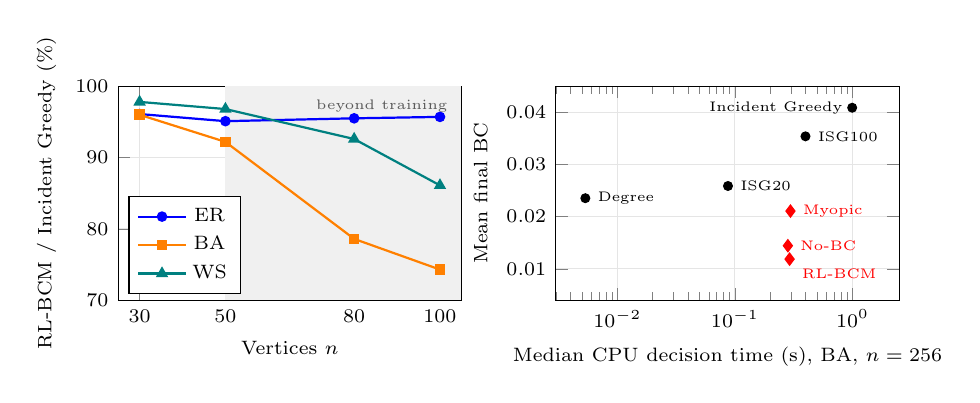
\begin{tikzpicture}
\begin{axis}[
  name=left, width=0.49\textwidth, height=4.3cm,
  xlabel={Vertices $n$}, ylabel={\rlbcm{} / Incident Greedy (\%)},
  xtick={30,50,80,100}, ymin=70, ymax=100, xmin=25, xmax=105,
  label style={font=\scriptsize}, tick label style={font=\scriptsize},
  legend style={font=\scriptsize, at={(0.03,0.03)}, anchor=south west},
  grid=major, grid style={gray!20}]
  \fill[gray!12] (axis cs:50,70) rectangle (axis cs:105,100);
  \node[font=\tiny, gray!70!black, anchor=north east] at (axis cs:104,99.5) {beyond training};
  \addplot[blue, thick, mark=*, mark size=1.5pt] coordinates {(30,96.1)(50,95.1)(80,95.5)(100,95.7)};
  \addplot[orange, thick, mark=square*, mark size=1.5pt] coordinates {(30,96.0)(50,92.2)(80,78.6)(100,74.3)};
  \addplot[teal, thick, mark=triangle*, mark size=1.8pt] coordinates {(30,97.8)(50,96.8)(80,92.6)(100,86.1)};
  \legend{ER, BA, WS}
\end{axis}
\begin{axis}[
  at={(left.east)}, anchor=west, xshift=1.2cm,
  width=0.49\textwidth, height=4.3cm, xmode=log,
  xlabel={Median CPU decision time (s), BA, $n=256$}, ylabel={Mean final BC},
  xmin=0.003, xmax=2.5, ymin=0.004, ymax=0.045,
  label style={font=\scriptsize}, tick label style={font=\scriptsize},
  yticklabel style={/pgf/number format/fixed, /pgf/number format/precision=2},
  scaled y ticks=false, grid=major, grid style={gray!20},
  nodes near coords, point meta=explicit symbolic,
  every node near coord/.append style={font=\tiny, anchor=west, xshift=1pt}]
  \addplot[only marks, mark=*, mark size=1.6pt, black] coordinates {
    (0.00534,0.02355) [Degree]
    (0.0873,0.02589) [ISG20]
    (0.3986,0.03540) [ISG100]
  };
  \addplot[only marks, mark=*, mark size=1.6pt, black,
    every node near coord/.append style={anchor=east, xshift=-1pt}]
    coordinates {(0.9950,0.04088) [Incident Greedy]};
  \addplot[only marks, mark=diamond*, mark size=2.2pt, red,
    every node near coord/.append style={red}] coordinates {
    (0.2823,0.01445) [No-BC]
    (0.2969,0.02108) [Myopic]
  };
  \addplot[only marks, mark=diamond*, mark size=2.2pt, red,
    every node near coord/.append style={red, anchor=north west}]
    coordinates {(0.2919,0.01188) [\rlbcm]};
\end{axis}
\end{tikzpicture}
\caption{Left: size transfer, as the ratio of \rlbcm's mean final BC to
Incident Greedy on the test set (training sizes are $n\le50$). Right:
quality versus CPU decision time on five BA graphs with $n=256$ (model
seed 11); search baselines in black, learned policies in red.}
\label{fig:main}
\end{figure}

Averages conceal a size effect (Fig.~\ref{fig:main}, left). Relative to
Incident Greedy, \rlbcm{} falls from 96.0\% at $n=30$ to 74.3\% at $n=100$
on BA and from 97.8\% to 86.1\% on WS, whereas ER stays near 95--96\%. The
losses thus arise mainly beyond the largest training size.

\subsection{Global features and the long-horizon objective}
\begin{table}[t]
\centering
\caption{Paired final-BC difference $\Delta$ (\rlbcm{} minus comparator),
crossed-bootstrap 95\% interval, percentage of paired seed-graph outcomes
won by \rlbcm, and Holm-corrected seed sign-flip $p$.}
\label{tab:contrasts}
\small
\setlength{\tabcolsep}{4pt}
\begin{tabular}{llrrrr}
\toprule
Family & Comparator & $\Delta$ & 95\% CI & Win (\%) & $p_H$ \\
\midrule
ER & Full Greedy & $-0.0035$ & $[-0.0048, -0.0023]$ & 6.5 & 0.188 \\
   & No-BC       & $+0.0016$ & $[+0.0006, +0.0027]$ & 63.7 & 0.188 \\
   & Myopic      & $-0.0008$ & $[-0.0018, +0.0001]$ & 34.0 & 0.188 \\
\midrule
BA & Full Greedy & $-0.0086$ & $[-0.0099, -0.0073]$ & 2.5 & 0.188 \\
   & No-BC       & $-0.0013$ & $[-0.0025, -0.0002]$ & 35.2 & 0.188 \\
   & Myopic      & $-0.0035$ & $[-0.0051, -0.0020]$ & 20.2 & 0.188 \\
\midrule
WS & Full Greedy & $-0.0184$ & $[-0.0224, -0.0145]$ & 11.5 & 0.188 \\
   & No-BC       & $+0.0047$ & $[-0.0041, +0.0140]$ & 46.5 & 0.500 \\
   & Myopic      & $-0.0039$ & $[-0.0112, +0.0049]$ & 32.5 & 0.438 \\
\bottomrule
\end{tabular}
\end{table}

Removing the BC input changes mean final BC by $-0.0016$, $+0.0013$, and
$-0.0047$ on ER, BA, and WS (Table~\ref{tab:contrasts}). Because the sign
is mixed, explicit BC features are not uniformly necessary. The
Myopic control obtains 0.0809, 0.0663, and 0.2678, exceeding \rlbcm{} in
all three family means. The experiments therefore do not show a
long-horizon advantage under our training budget. Optimization difficulty,
or the strength of immediate gains for peripheral targets, may explain
this, but neither mechanism was measured.

\subsection{Exact optima and budget transfer}
\label{sec:diagnostics}
On the 60 eight-vertex graphs with $k=2$, which are smaller than any
training graph, Full Greedy is suboptimal on 6 graphs (mean final BC 0.1583 versus optimum 0.1594). \rlbcm{} averages
0.1188 and reaches the optimum in 46.3\% of the 300 seed-graph outcomes.
This pooled rate hides family rates of 22\% (ER), 22\% (BA), and 95\% (WS).
On the six graphs where greedy is suboptimal, \rlbcm{} beats greedy and
attains the optimum in only 1 of 30 outcomes. A disjoint set of six graphs
(five WS, one BA) has fewer than two incident non-edges, so Incident Greedy
is infeasible there. Without retraining, on the 60 test graphs with $n=50$, the mean final BC of
\rlbcm{}/Full Greedy is 0.0348/0.0415 at $k=1$, 0.0900/0.0966 at $k=3$, and
0.2350/0.2408 at $k=10$. Since the budget feature $b_t/k$ equals one at the
start of every horizon, this transfer test has limited resolution.

\subsection{Real-network transfer}
\begin{table}[t]
\centering
\caption{Mean final BC on real networks: three subgraphs (or LCC targets)
per row; ISG20/ISG100 and learned models average five seeds. Dashes denote
methods not run at that size. On 80-vertex samples Full Greedy equals
Incident Greedy. On GrQc BFS~256, Degree and No-BC differ in
the fifth decimal (0.06080 vs.\ 0.06081).}
\label{tab:real}
\small
\setlength{\tabcolsep}{4pt}
\begin{tabular}{lrrrrrr}
\toprule
Network / sample & Degree & ISG20 & ISG100 & \shortstack{Incident\\Greedy} & \rlbcm & No-BC \\
\midrule
Email BFS 80   & 0.0047 & 0.0132 & 0.0137 & 0.0137 & 0.0121 & 0.0115 \\
Email RW 80    & 0.0020 & 0.0287 & 0.0337 & 0.0337 & 0.0304 & 0.0268 \\
Email BFS 256  & 0.0004 & 0.0062 & 0.0089 & 0.0096 & 0.0072 & 0.0068 \\
Email RW 256   & 0.0008 & 0.0042 & 0.0062 & 0.0067 & 0.0050 & 0.0050 \\
Email LCC 986  & 0.0002 & 0.0031 & 0.0058 & --     & \textbf{0.0061} & 0.0053 \\
\midrule
GrQc BFS 80    & 0.2838 & 0.2808 & 0.3168 & 0.3168 & 0.2720 & 0.2518 \\
GrQc RW 80     & 0.2463 & 0.4687 & 0.5032 & 0.5032 & 0.3520 & 0.3651 \\
GrQc BFS 256   & 0.0608 & 0.0700 & 0.1196 & 0.1386 & 0.0398 & 0.0608 \\
GrQc RW 256    & 0.0046 & 0.2811 & 0.3234 & 0.3415 & 0.1553 & 0.1543 \\
GrQc LCC 4158  & 0.0042 & 0.0195 & 0.0297 & --     & 0.0072 & 0.0092 \\
\bottomrule
\end{tabular}
\end{table}

Table~\ref{tab:real} contains the clearest positive result. On the full
986-vertex email-Eu-core LCC, \rlbcm{} attains 0.0061, above ISG100
(0.0058) and ISG20 (0.0031), although this rests on only three targets.
Transfer to ca-GrQc is poor. There, ISG20/ISG100 reach 0.0195/0.0297 on the LCC
versus 0.0072 for \rlbcm, and on BFS-256 subgraphs \rlbcm{} attains 0.0398
versus 0.1386 for Incident Greedy. All BC values are normalized within the
optimized graph, so subgraph BC is not the BC in the source network.

\subsection{Decision cost}
\begin{table}[t]
\centering
\caption{Quality and cost at $n=256$: mean final BC (top) and median CPU
decision time in seconds (bottom) on five graphs per family, three
repetitions, one thread, model seed 11.}
\label{tab:timing}
\small
\setlength{\tabcolsep}{3.5pt}
\begin{tabular}{lrrrrrrr}
\toprule
Family & Degree & ISG20 & ISG100 & \shortstack{Incident\\Greedy} & \rlbcm & No-BC & Myopic \\
\midrule
ER & \shortstack[r]{0.0026\\{\scriptsize 0.0055}} & \shortstack[r]{0.0036\\{\scriptsize 0.1042}} & \shortstack[r]{0.0038\\{\scriptsize 0.4188}} & \shortstack[r]{0.0038\\{\scriptsize 0.9696}} & \shortstack[r]{0.0037\\{\scriptsize 0.3118}} & \shortstack[r]{0.0037\\{\scriptsize 0.2690}} & \shortstack[r]{0.0038\\{\scriptsize 0.3051}} \\
BA & \shortstack[r]{0.0236\\{\scriptsize 0.0053}} & \shortstack[r]{0.0259\\{\scriptsize 0.0873}} & \shortstack[r]{0.0354\\{\scriptsize 0.3986}} & \shortstack[r]{0.0409\\{\scriptsize 0.9950}} & \shortstack[r]{0.0119\\{\scriptsize 0.2919}} & \shortstack[r]{0.0144\\{\scriptsize 0.2823}} & \shortstack[r]{0.0211\\{\scriptsize 0.2969}} \\
WS & \shortstack[r]{0.2518\\{\scriptsize 0.0057}} & \shortstack[r]{0.3016\\{\scriptsize 0.0905}} & \shortstack[r]{0.3235\\{\scriptsize 0.4139}} & \shortstack[r]{0.3463\\{\scriptsize 0.9997}} & \shortstack[r]{0.2636\\{\scriptsize 0.3068}} & \shortstack[r]{0.2198\\{\scriptsize 0.2889}} & \shortstack[r]{0.2953\\{\scriptsize 0.3153}} \\
\bottomrule
\end{tabular}
\end{table}

Table~\ref{tab:timing} and Fig.~\ref{fig:main} (right) pair quality and
time on identical graphs. Across the nine family-size cells of the timing
benchmark, another method has both higher mean BC and lower median time
than \rlbcm{} in eight. For example, on BA-256, ISG20 attains 0.0259 in
0.087\,s versus 0.0119 in 0.292\,s for \rlbcm. The exception is ER-100,
where \rlbcm{} attains 0.0208 in 0.048\,s versus 0.0217 in 0.059\,s for
Incident Greedy, a small speedup at slightly lower quality. Training the
five \rlbcm{} models took 37.1 cumulative CPU process-minutes, which would
only be amortized by many uses with positive latency savings.

%======================================================================
\section{Conclusion}
\label{sec:conclusion}
\rlbcm{} learns a useful heuristic that beats degree and global sampled
search. On our synthetic benchmark, however, exact and sampled incident
search reach higher quality, and so does the myopic control. The quality
of \rlbcm{} also drops beyond the training sizes. The results are limited to low-BC
targets, one training corpus, five seeds, and two real networks. Future
learned policies should score only the $O(n)$ incident candidates instead
of all $O(n^2)$ missing edges, since incident edges suffice for optimality,
and be evaluated against incident search on new holdout sets, especially
at larger sizes.

\paragraph{Code and data availability.}
Code and results are available at \codeurl, including
every graph-target instance, the 15 trained checkpoints with training
histories, per-step trajectories, raw measurements, and a detailed
experimental report.

\bibliographystyle{splncs04}
\bibliography{references}
\end{document}
